\documentclass[a4 paper,12pt]{article}
\usepackage[margin=1.3cm]{geometry}
\usepackage{graphicx}
\title{\bfseries\Huge Controlling FireBird-V Robot using EEG sensor}
\author{\textbf{Step wise study report on the project}}
\date{}


\begin{document}
	\begin{minipage}{0.95\textwidth}
		\begingroup
		\let\endcenter\endflushleft
		\maketitle
		\endgroup
	\end{minipage}
	

\begin{minipage}{0.98\textwidth}
		\section{What is EEG?...}
		\vspace{-0.1in}
		Electroencephalography (EEG) is a non-invasive method to record electrical activity of the brain along the scalp. EEG measures voltage fluctuations resulting from ionic current within the neurons of the brain. In clinical contexts, EEG refers to the recording of the brain's spontaneous electrical activity over a period of time, as recorded from multiple electrodes placed on the scalp.\\\\The brain's electrical charge is maintained by billions of neurons. Neurons are electrically charged (or "polarized") by membrane transport proteins that pump ions across their membranes. Neurons are constantly exchanging ions with the extracellular milieu, for example to maintain resting potential and to propagate action potentials. Ions of similar charge repel each other, and when many ions are pushed out of many neurons at the same time, they can push their neighbours, who push their neighbours, and so on, in a wave. This process is known as volume conduction. When the wave of ions reaches the electrodes on the scalp, they can push or pull electrons on the metal on the electrodes. Since metal conducts the push and pull of electrons easily, the difference in push or pull voltages between any two electrodes can be measured by a voltmeter. Recording these voltages over time gives us the EEG.\\\\The electric potential generated by an individual neuron is far too small to be picked up by EEG. EEG activity therefore always reflects the summation of the synchronous activity of thousands or millions of neurons that have similar spatial orientation. If the cells do not have similar spatial orientation, their ions do not line up and create waves to be detected. Pyramidal neurons of the cortex are thought to produce the most EEG signal because they are well-aligned and fire together. Because voltage fields fall off with the square of distance, activity from deep sources is more difficult to detect than currents near the skull.\\\\Scalp EEG activity shows oscillations at a variety of frequencies. Several of these oscillations have characteristic frequency ranges, spatial distributions and are associated with different states of brain functioning (e.g., waking and the various sleep stages). These oscillations represent synchronized activity over a network of neurons. The neuronal networks underlying some of these oscillations are understood (e.g., the thalamocortical resonance underlying sleep spindles), while many others are not (e.g., the system that generates the posterior basic rhythm). Research that measures both EEG and neuron spiking finds the relationship between the two is complex, with a combination of EEG power in the gamma band and phase in the delta band relating most strongly to neuron spike activity.\\\\
\end{minipage}
	
	
\begin{minipage}{0.98\textwidth}
	\section{About EEG sensor(Mindwave Mobile Headset)}
	\vspace{-0.1in}
Measuring EEG* activity has traditionally required complex equipment costing thousands of dollars. Now, with our research-grade, embeddable biosensor, NeuroSky has unlocked a new world of affordable solutions for health and wellness, education and entertainment. Precisely accurate, portable, and noise filtering, our EEG biosensors collect electrical signals — not actual thoughts — to translate brain activity into action.\\\\NeuroSky’s EEG biosensor digitizes and amplifies raw analog brain signals to deliver concise inputs to games, toys, and devices running health and wellness, educational and research applications. Our brainwave algorithms, developed by NeuroSky neuroscientists and our partner research institutions, have revealed many new ways to interact with our world.\\\\\textbf{EEG Biosensors Features}\\
Direct connect to dry electrode, One EEG channel + Reference + Ground, Extremely low-level signal detection, Advanced filter with high noise immunity, RAW EEG at 512Hz\\
\textbf{eSense Brainwave Patterns}\\
RAW EEG Signal, Attention, Meditation, Eye Blink, Delta, Theta, low apha, high alpha, low beta, high beta and gamma waves\\
\textbf{Dimensions}\\
Size: 2.79cm x 1.52cm x 0.25cm\\Weight (Max) 130mg\\
\textbf{Specifications}\\
512Hz sampling rate\\
3-100Hz frequency range\\
ESD Protection: 4kV Contact Discharge; 8kV Air\\
Max Power Consumption: 15mA @ 3.3V • Operating voltage 2.97 ~3.63V\\
\textbf{UART (Serial):}\\
1200, 9600, 57600 baud, 8-bits, No parity, 1 stop bit
\end{minipage}
\begin{center}
	\graphicspath{ {images/} }
	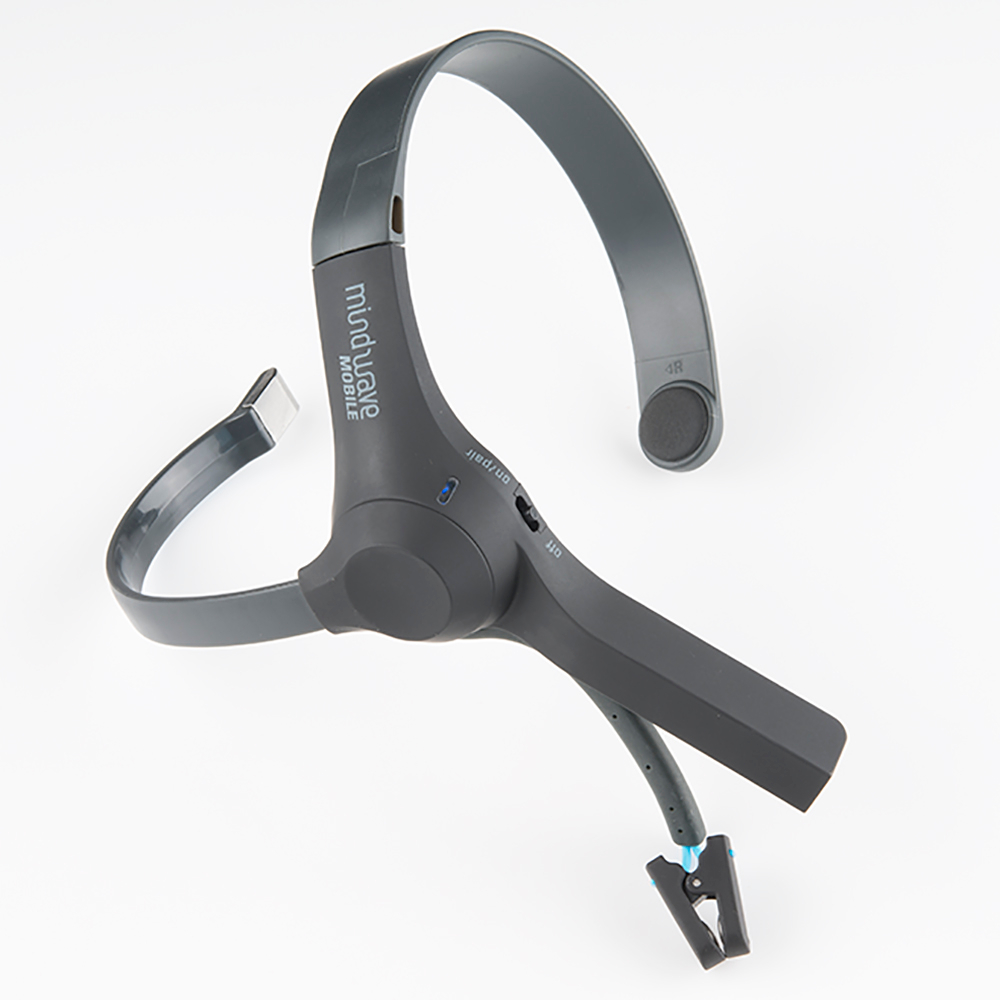
\includegraphics[width=12cm, height=10cm]{Mindwave_mobile}
\end{center}

\begin{minipage}{0.98\textwidth}
	\section{How EEG sends data?...}
	\vspace{-0.1in}
ThinkGear components deliver their digital data as an asynchronous serial stream of bytes. The serial
stream must be parsed and interpreted as ThinkGear Packets:\\1. Packet Header\\2. Packet Payload\\3. Payload Checksum\\\textbf{Packet Structure}\\-----------------Header------------------------------Payload--------------------Checksum-----\\
--[SYNC][SYNC][PayloadLength]------[PAYLOAD DATA...]------[CHECKSUM]--\\\\\textbf{Packet Header}\\
The two [SYNC] bytes are used to signal the beginning of a new arriving Packet and are bytes with
the value 0xAA (decimal 170). Synchronization is two bytes long, instead of only one, to reduce the
chance that [SYNC] (0xAA) bytes occurring within the Packet could be mistaken for the beginning of
a Packet.\\The [PLENGTH] byte indicates the length, in bytes, of the Packet's Data Payload [PAYLOAD…]
section, and may be any value from 0 up to 169. Any higher value indicates an error (PLENGTH TOO
LARGE). Be sure to note that [PLENGTH] is the length of the Packet's Data Payload, NOT of the
entire Packet. The Packet's complete length will always be [PayloadLength] + 4.\\\\
\textbf{Data Payload}\\The Data Payload of a Packet is simply a series of bytes. The number of Data Payload bytes in the
Packet is given by the [PLENGTH] byte from the Packet Header.\\\\\textbf{Payload Checksum}\\The [CHKSUM] Byte must be used to verify the integrity of the Packet's Data Payload. The Payload's
Checksum is defined as:\\
1. summing all the bytes of the Packet's Data Payload\\
2. taking the lowest 8 bits of the sum\\
3. performing the bit inverse (one's compliment inverse) on those lowest 8 bits\\\\  
\textbf{Step-By-Step Guide to Parsing a Packet}\\
\textbf{1.} Keep reading bytes from the stream until a [SYNC] byte (0xAA) is encountered.\\
\textbf{2.} Read the next byte and ensure it is also a [SYNC] byte, If not a [SYNC] byte, return to step 1., Otherwise, continue to step 3.\\
\textbf{3.} Read the next byte from the stream as the [PLENGTH].,  If [PLENGTH] is 170 ([SYNC]), then repeat step 3., If [PLENGTH] is greater than 170, then return to step 1 (PLENGTH TOO LARGE)., Otherwise, continue to step 4.\\
\textbf{4.} Read the next [PLENGTH] bytes of the [PAYLOAD…] from the stream, saving them into a storage area (such as an unsigned char payload[256] array). Sum up each byte as it is read by
incrementing a checksum accumulator (checksum += byte).\\
\textbf{5.} Take the lowest 8 bits of the checksum accumulator and invert them.\\
\textbf{6.} Read the next byte from the stream as the[CHKSUM] byte., If the [CHKSUM] does not match your calculated chksum (CHKSUM FAILED)., Otherwise, you may now parse the contents of the Payload into DataRows to obtain the Data
Values, as described below., In either case, return to step 1.\\\\
\end{minipage}
	
\end{document}
	